%Kinwalker_Bac - Progress report
\documentclass{beamer}
\usepackage{graphicx}
\usepackage{amsmath,amsfonts,amssymb}
%exclude navigation symbols
\beamertemplatenavigationsymbolsempty
\usetheme[compress]{Dresden}
\usecolortheme{seagull}
\usefonttheme{structurebold}
\expandafter\def\expandafter\insertshorttitle\expandafter{\insertshorttitle\hfill\insertframenumber\,/\,\inserttotalframenumber}

\title[Kinwalker parameter space analysis]{Kinwalker parameter space analysis}

\author[Mario Koestl]{Mario Koestl}
\institute[TBI]{Institute for Theoretical Chemistry\\ University of Vienna}
\date{\today}
\subject{}
\keywords{}
%\newcommand{\TODO}[1]{{\color{red} #1}}
\begin{document}
\frame{
  \titlepage
}


\frame{
\frametitle{Overview}

\begin{itemize}
\item co-transcriptional folding = RNA folding at the growing 5' end
\item co-transcriptional pathway prediction difficult
\item Kinwalker algorithm: heuristic approach for RNA folding kinetic prediction
\end{itemize}

}

%-- cotranscriptional folding, difficult to predict, faltungkinetic teuer, darum kinwalker

%During transcription the new RNA strand is created starting with the 5' end, therefore RNA folding can occur at the growing 5' end\cite{Kramer1981}.
%In contrast to MFE prediction, computing co-transcriptional pathways of secondary structures is extremely difficult. Only a handful of programs allow for an efficient prediction. The program Kinwalker is one of them, and aims to substitute the effort of predicting RNA folding kinetics, by a heuristic approach, that deterministically follows the most probable trajectory folding. 
%
% 
% %-- kurze Kinwalker beschreibung, Pfandfindungsheuristiken, zwischenstrukturen wechseln, Laenge der max, structuren
%

\frame{
\frametitle{Kinwalker}
\begin{itemize}

\item predicts secondary structure trajectories up to 1500 nt
\item uses structures backtracked from $C_{i,j}$ matrix after each base adding step.
\item 2 direct pathfinding algorithm : "Morgan Higgs" and "findpath" 

\end{itemize}
}

%
%One of the first steps of the Kinwalker algorithm is to create a $C_{i,j}$ matrix. This matrix consists of MFE values ranging from base position i to j. To calculate this matrix, every possible $(x_i,...,x_j)$ sub-sequence is taken and their MFE structure is calculated. 
%Every cycle of transcription adds one base to the growing RNA strand, therefore sequences with different length are present during transcription. At the beginning of each step we have the current i-j structure and have to find a way to the i-j+1 structure. To do so, \texttt{Kinwalker} makes use of all the MFE substructures backtracked from the $C_{i,j}$ matrix. Every possible substructure is used as a candidate that might be merged into the structure trajectory. To find the best path between these 2 structures Kinwalker has implemented two direct path-finding algorithms. The first one is the Morgan Higgs algorithm (implemented by Morgan and Higgs) and the second one is the findpath algorithm (implemented by Christoph Flamm). Both of these methods are heuristics, since the general problem of finding direct paths is NP hard.
%
%The Kinwalker algorithm is able to predict secondary structure trajectories of RNA sequences up to 1500 nucleotides in length. 
%
%
%
%%-- Parameter des Kinwalkers, nicht dangle erklaehren

\frame{
\frametitle{Kinwalker parameters used}


\begin{itemize}
\item transcription rate
\item barrier heuristic
\item dangle model
\item max keep
\end{itemize}

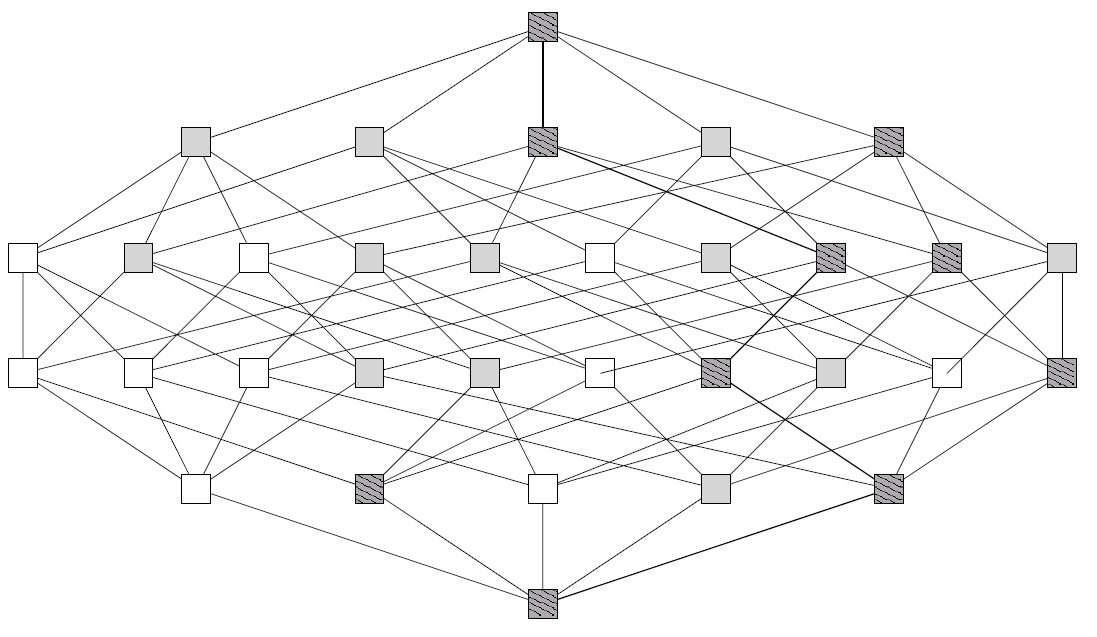
\includegraphics[width=0.6\textwidth]{./pictures/find-path.png} 


}

%For fine tuning of the Kinwalker algorithm different parameters are available. For my parameter space analysis, I only used transcription rate, barrier heuristic, dangle model and max keep. Transcription rate is the number of nucleotides transcribed by the RNA polymerase per second. 
%Transforming, i.e. adding or deleting substructures backtracked from the $C_{i,j}$ matrix, consumes time. 
%If Kinwalker tries to insert a new substructure, the corresponding energy barrier is checked if such insertion could be even possible within the given time. If the energy barrier was to high, and therefore the time was to short, this specific substructure cannot be inserted and another one is tried.
%
%Morgan-Higgs and find-path algorithm are similar, but differ at choosing the best path. Morgan-Higgs is based on minimal collisions between the i-j structure and i-j+1 structure and find-path is based on minimal free energy differences. Furthermore, find-path uses a breadth-first search, and is therefore able to examine more than one solution path.

%Dangle model is the used energy model for adjacent dangling bases and max keep is the amount of searched paths in the breadth-first search of findpath.

%
%
%%--Effect der Paraemter, Datensaetze genommen
%%--Welche Datensaetze
%


\frame{
\frametitle{data used}

\begin{itemize}

\item 200 different parameter combinations for 3 RNA families
\item SRP, TRP and RNAseP
\item alignment for each family from Rfam database, according to Meyer et al.
\item reference structures taken from literature, reference sequences downloaded from NCBI

\end{itemize}
}



%To compare parameter changes, a total of 200 different parameter combinations were tried over well studied sequences. 
%
%The signal recognition particle (SRP)\cite{SRP}, tryptophan leader transcript (TRP)\cite{sourceRefTRP} and the bacterial ribonuclease P (RNAseP)\cite{RNAseP} are used for calculations, because they are well studied RNA classes with existing benchmark studies. Furthermore, for this families, some reference structures and partial co-transcriptional folding intermediates are available. 
%
%The original alignment data for each RNA class was obtained from the Rfam database, according to Meyer et al.\citep{Meyer}. 
%Reference structures were taken from literature and reference sequences were downloaded from \texttt{NCBI database} in FASTA format. 
%
%%--Scores, Fuer vergleiche diese scores verwenet-- einfach auflisten.

\frame{
\frametitle{Scoring functions}
\begin{itemize}

\item comparing Kinwalker output data with different parameters
\item Structure Conservation Index and Sequence Similarity
\item Base-pair diversity, ensemble diversity, ensemble distance

\end{itemize}
}


%Different scoring functions were used to compare Kinwalker output data of different parameters.
%I used the Structure conservation index and the sequence similarity to analyse the input alignment data and for kinwalker outputs I used the base-pair diversity, the ensemble diversity or the ensemble distance to a reference structure.


\frame{
\frametitle{ensemble distance}

\begin{itemize}

\item expected distance between folding trajectory and a reference structure



 \begin{equation}
\mbox{ensemble distance(s,ref)} = \sum\limits_{i,j \in ref } (1- p(i,j)) + \sum\limits_{i,j \notin ref} p(i,j),
\label{eq:ensemble distance}
\end{equation}

\item $p(i,j) = \frac{\Delta Time}{T_{total}}$.
\end{itemize}
}

%
%
%% --> Ensemble Distance genauer erklaehren, auch als Bild. was ist P(i,j)
%The ensemble distance is the expected distance between the predicted trajectory of one sequence and a reference structure. 
%
%
% is the probability of appearance of $(i,j)_{s}$ in the folding trajectory. $\Delta$Time is the existence time of one base-pair during the whole RNA folding event. $T_{total}$ is the time until the RNA is fully transcribed and has successfully folded into the MFE structure.
%
%
%
%%--Interessante Bilder
%%-- Des midn Peak

\frame{
\frametitle{Results}
\begin{figure}
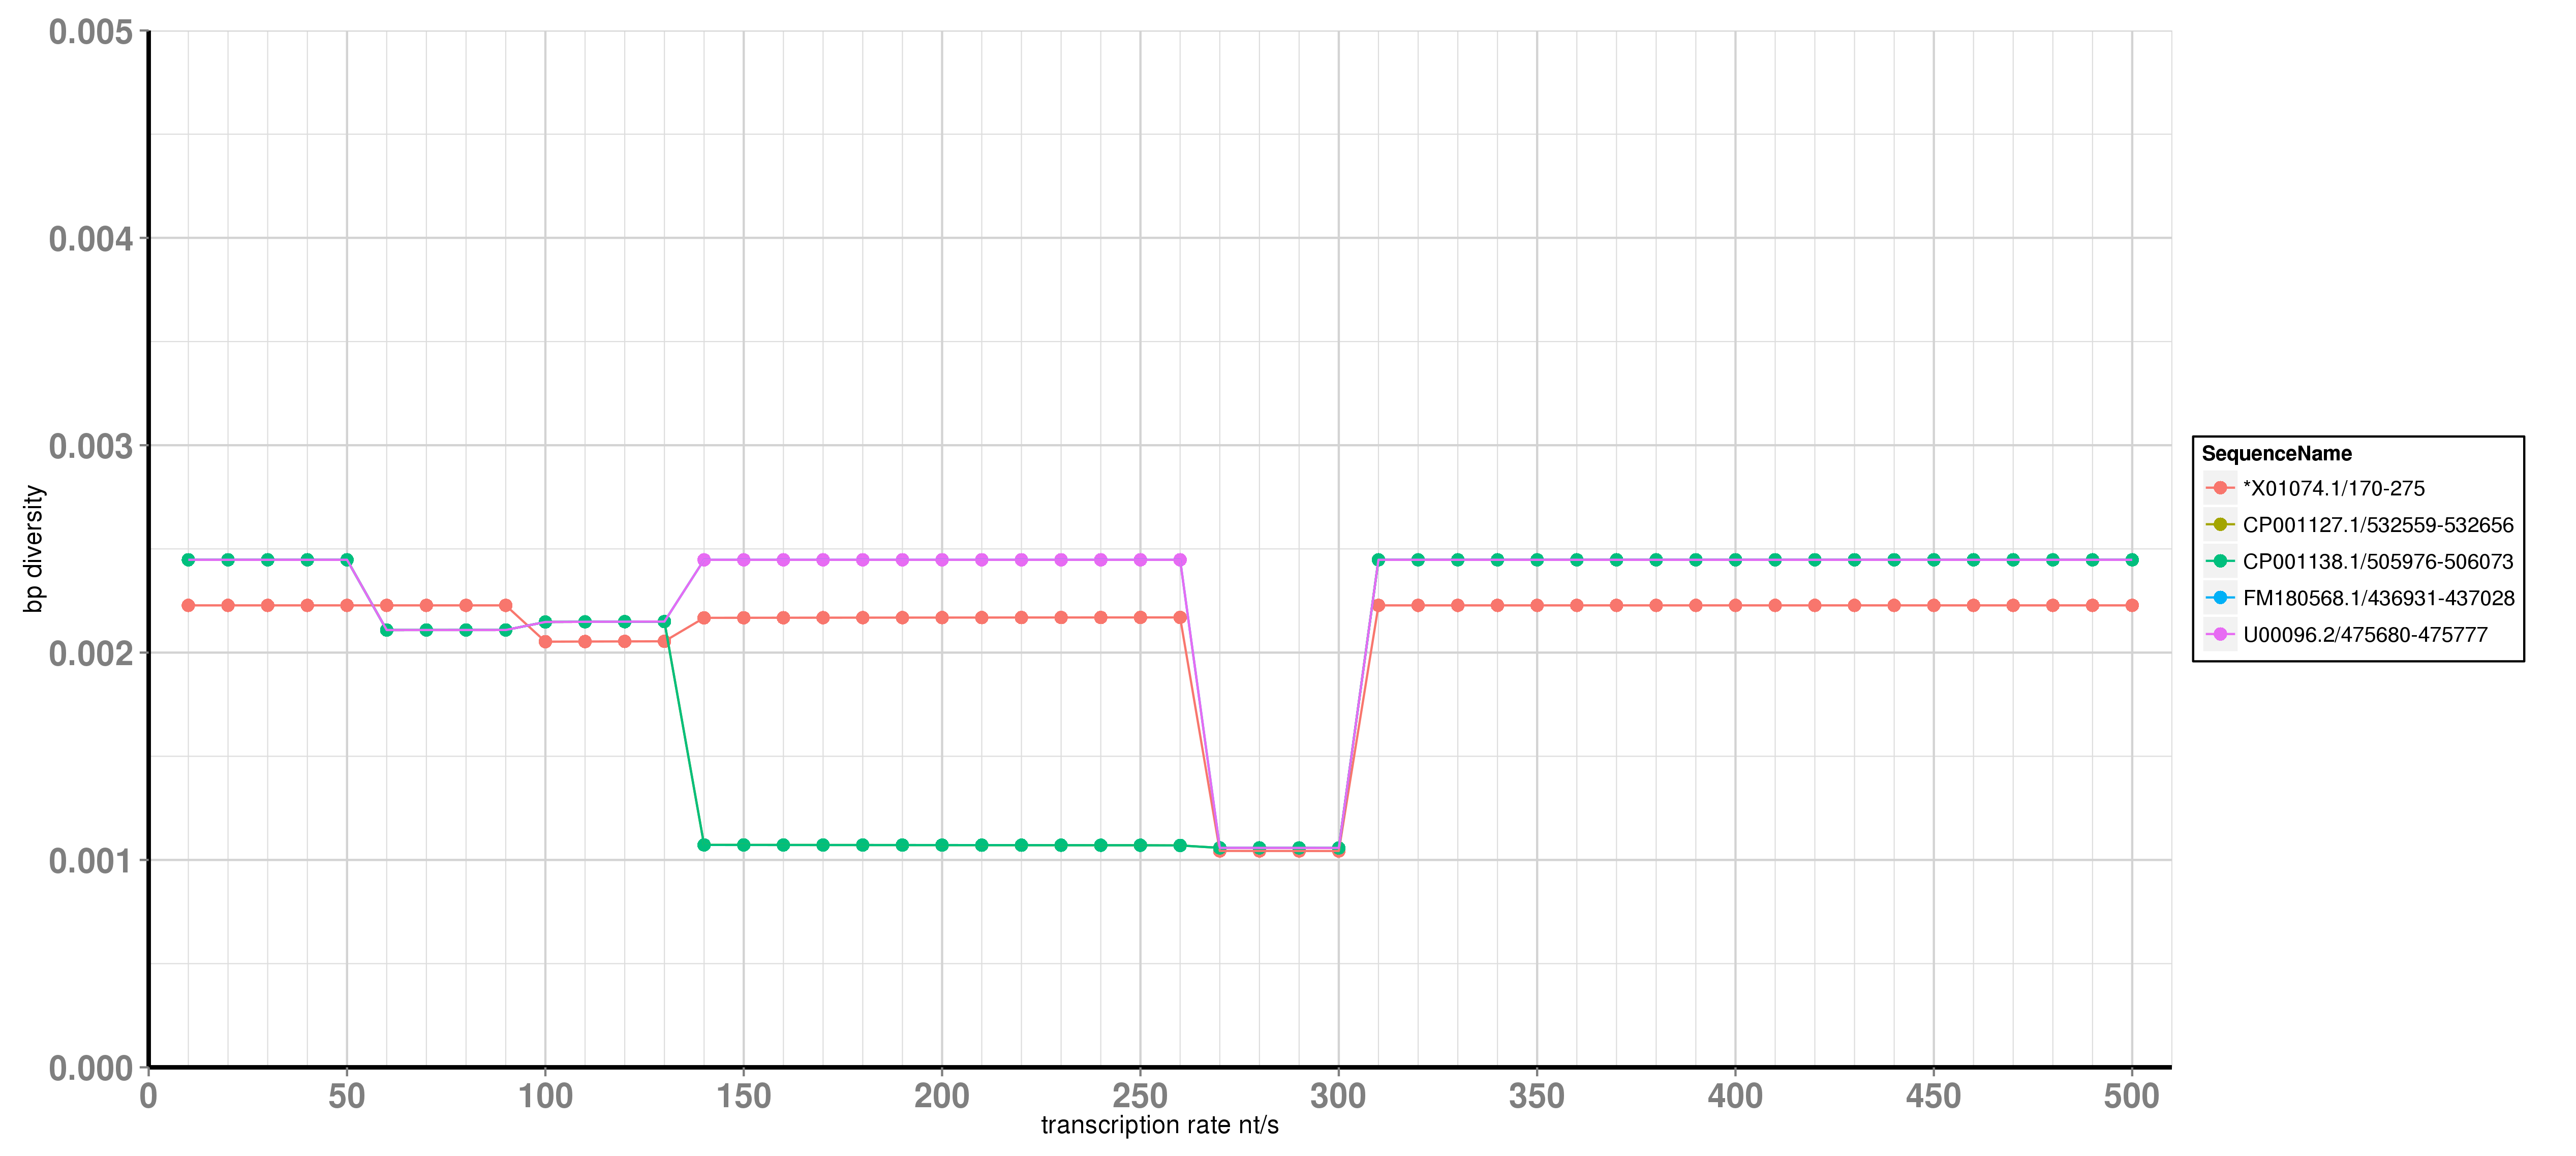
\includegraphics[width=0.7\textwidth]{./pictures/Discussion_results/SRP/SRPseqDecrease250_300nts.png}

\tiny{

\begin{tabular}{l|l|l|l}
sequence & trap at 260 nt/s  & trap at 300 nt/s & trap at 310 nt/s\\
\hline
X01074.1.170-275			&	yes &	no	&	yes \\
U00096.2.475680-475777		&	yes	&	no	&	yes	\\
FM180568.1.436931-437028	&	yes	&	no	&	yes	\\
CP001138.1.505976-506073	&	yes	&	no	&	yes	\\
CP001127.1.532559-532656 	&	no	&	no	&	yes	\\
\end{tabular}	


}
\end{figure}

}


%
%
%This diagram shows the bp diversity for 5 SRP family sequences, which have a common base-pair diversity drop at transcription rates of 270-300 nt/s.
%The X axis shows the used transcription rates ranging from 10 to 500 with steps of 10 and on the Y axis is the calculated base-pair diversity shown.
%
%Furthermore this sequences are forming a folding trap at every other transcription rates and are forming directly into their MFE structures inside this drop basket. 

\frame{
\frametitle{}
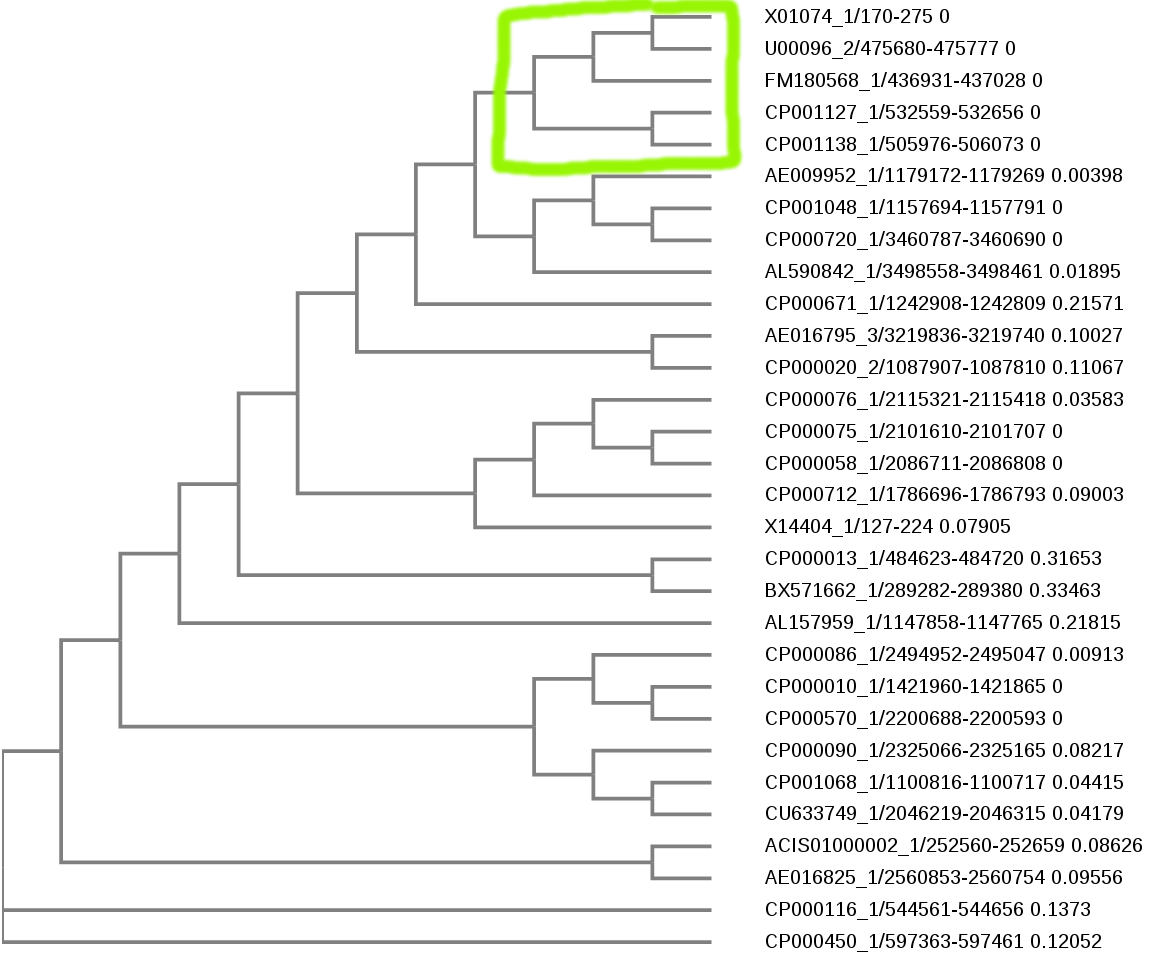
\includegraphics[width=0.5\textwidth]{./pictures/Discussion_results/SRP/srp_pylotree_edited.png}
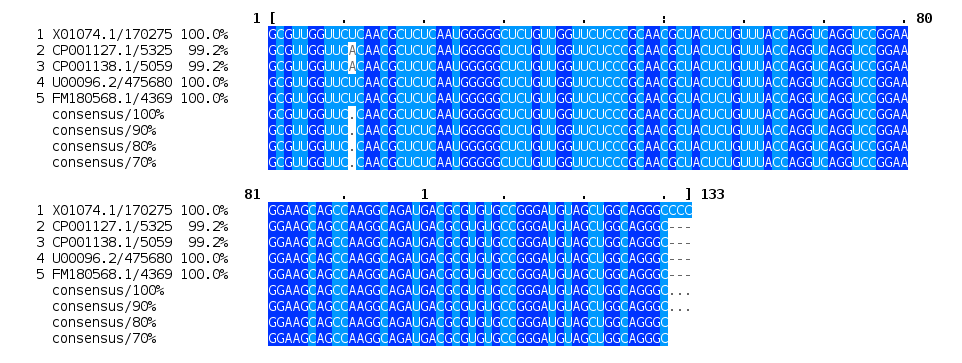
\includegraphics[width=0.5\textwidth]{./pictures/Discussion_results/SRP/MSA_SRP_5seq.png}
}
%Sadly, this sequences are nearly similar if aligned and therefore this sequence behavior is no evidence for co-transcriptional folding conservation but rather for evolutionary sequence conservation.

%
%
%
%%TRP als negativ beispiel


\frame{
\frametitle{TRP family}

\begin{itemize}
\item Ensemble Distance for trp sequences to terminator structure

\end{itemize}
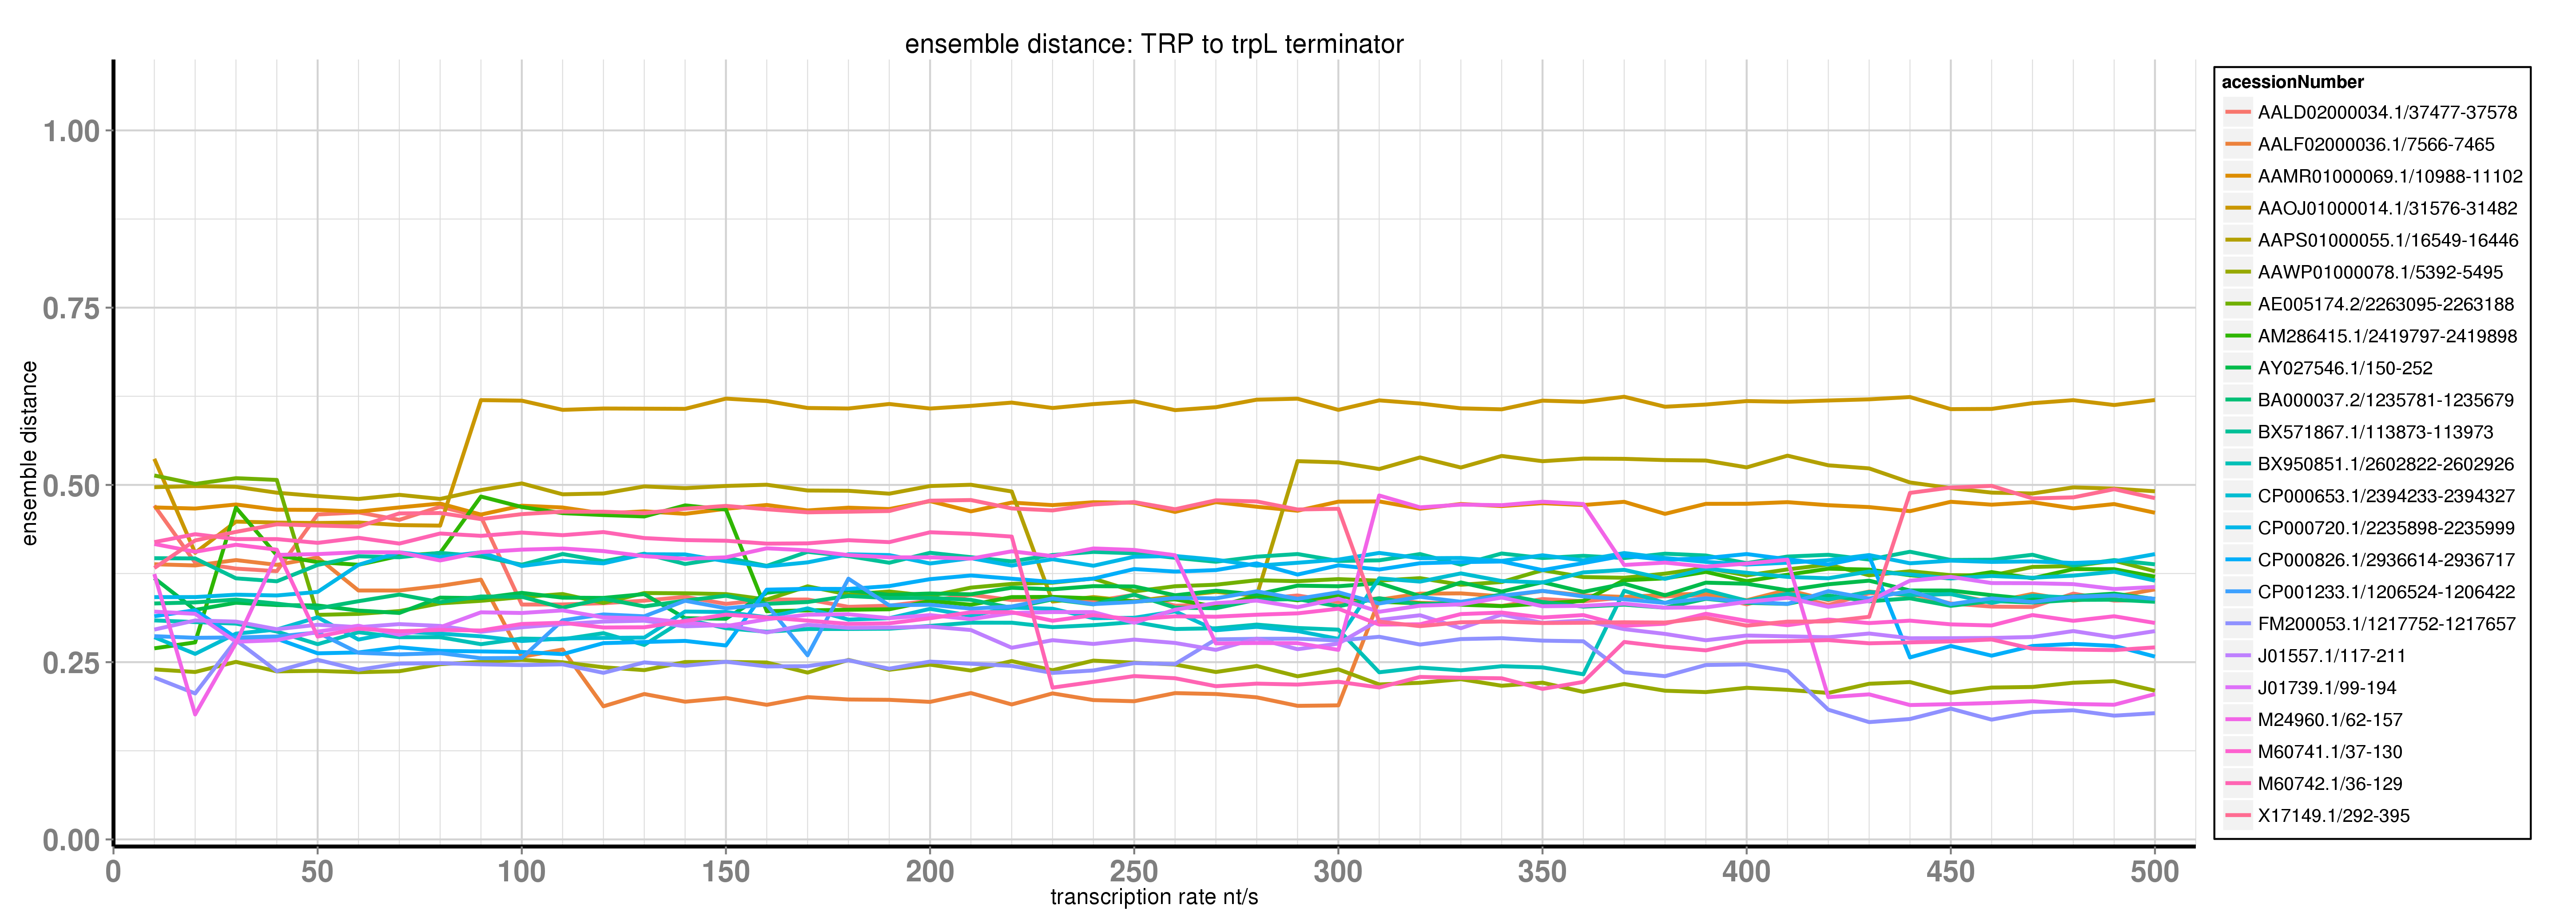
\includegraphics[width=1\textwidth]{./pictures/Discussion_results/TRP/ensembleDistance_terminator.png}


}

%
%I used the TRP family to analyse 
%
%
%Ensemble Distances from every TRP trajectory to the trpL terminator hairpin, is used to determine the distance to the terminator hairpin throughout the transcription rates. According to figure:~\ref{fig:trp_Terminator_ensembleDistance}, no noteworthy dependencies are apparent. Some sequences are rather forming the terminator hairpin at low transcription rates, others on higher rates. Evidence for increased probability of terminator formation with lower transcription rates or vica verse cannot be obtained. 
%I conclude, that with my used methods, significant influence of transcription rate to the formation of the terminator hairpin cannot be shown.  For further studies, extended transcription rates or different scores should be tried.
%

\frame{
\frametitle{conclusion}
blablabla, auch was das es halt icht geht
}

\end{document}

